\section{Related Work}
\label{sec:background-related-work}


{\bf Open source hardware and software are increasingly used on low-cost CubeSats}, including on microcontroller parts.
For instance pyCubed~\cite{Holliday2019PyCubed} proposes open source CubeSat hardware based on an Arm Cortex-M4 (atsamd51) microcontroller and corresponding open source software based on Python (Adafruit CircuitPython).
OreSat~\cite{spivey2021oresat} designs a CubeSat also based on microcontrollers, and provides corresponding open source software.
Oragnisations such as the Libre Space Foundation~\cite{librespace} harbor a number of open source software code basis for CubeSats, such as UPSat, Qubik. 

Once the CubeSat is in orbit, during its lifetime, the software it embarks must typically be updated over-the-air.
Some work such as~\cite{FitzsimmonsReliableSoftwareUpdates} has focused on the reliability of the ground-flight link for CubeSat firmware updates.
Other work has focused on mitigating radiation effects corrupting firmware storage and on error correction, such as in \cite{yuen2019low} or partly in \cite{sunter2016updatesnano}.
A vanilla approach to securing low-cost CubeSat software updates, such as described in~\cite{maison2021otaeducubesat}, only uses weak security primitives (e.g., MD5 integrity checks) instead of strong primitives such as authentication with digital signatures and encryption.
However, recent cyberattacks such as the ViaSat outage in Ukraine~\cite{viasat-cyberattack} suggest that, as CubeSat systems become more popular, they are likely to also become more prone to cyberattacks.
A crucial related challenge is thus {\bf how to provide strong security for software updates} while in orbit.
Prior work such as NUTS~\cite{birkeland2014nutsoverview,bezem2013nutsAuthenticatedUplink} has focused on authentication and communication security over the ground-flight uplink for firmware updates.

To the best of our knowledge, however, no prior work exists on providing strong security for software updates on a low-power CubeSat \textit{payload}, via a satellite uplink and an OBC that are \textit{both potentially untrusted}.
This hosted CubeSat use-case is depicted in \autoref{fig:e2e}.



\begin{figure}[t]
    \centering
    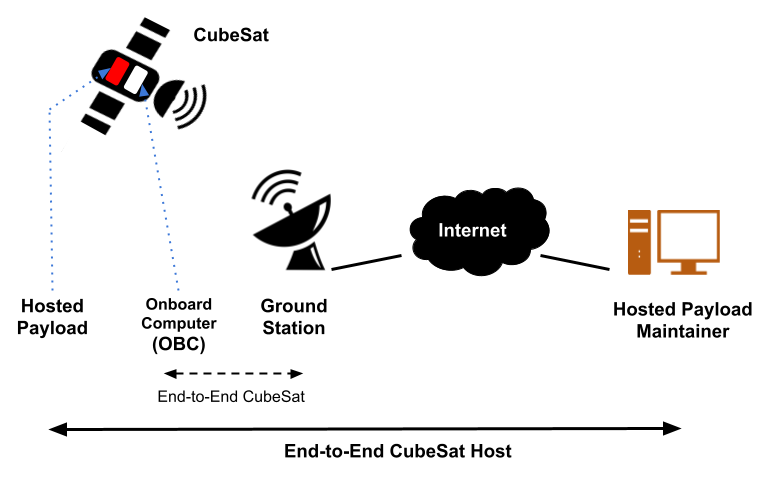
\includegraphics[width=0.5\textwidth]{Figures/CubeSat-Payload-End2End.png}
    \caption{CubeSat hosted payload software update security end-to-end.}
    \label{fig:e2e}
\end{figure}


\iffalse

\subsection{CubeSat Software Updates}
\label{sec:fu-cubesat}
\textit{Microcontroller}: studies issues related to firmware updates of in orbit
satellite subsystems \cite{sunter2016updatesnano}.\\
\textit{Linux systems}: most of the work in literature has focused on OBC firmware
updates, which tend to be linux systems. Most solutions target on-board storage
and error correction. E.g.: \cite{FitzsimmonsReliableSoftwareUpdates} focuses on
reliability of updates.\\
\textit{Securing Satellites Uplink}: NUTS (NTNU Test Satellite)\cite{birkeland2014nutsoverview}
research is focused on authenticated and secure uplinks for ground-flight communication but
uses mainly symmetric cryptography. Uses CSP. Authentication is HMAC challenge
\cite{Muench2014IntegrationAV} based using timestamps \cite{bezem2013nutsAuthenticatedUplink}.
\cite{yasir2021EncryptioUnitSat} secure communication via encryption with AES, diffie-hellman
and HMAC, its tested on atmega32.\\
\textit{OTA for Educational CubeSat}\cite{maison2021otaeducubesat}: uses MD5 for
authentication based on the fact that there will be a limited amount of messages.
Does not use public key signing because it makes for messages that look like encrypted
data, frowned upon in radio-amateurs community. Modifies linker script to achieve
small firmware payloads and targeted updates.\\
\textit{Firmware Updating Systems for nanosatellites}\cite{sunter2016updatesnano}:
stm32f103, stm32217, atmega1280, msp420, using FreeRtos, TinyOS and baremetal. Focused
on retransmissions, re-ordering schemes and image backups.\\

\subsection{CubeSat Open Source Software}
\label{sec:open-source-cubesat}
\textit{pyCubed}:\cite{Holliday2019PyCubed}: OpenSource CircuitPython based CubeSat
ecosystem: hardware and software. CORTEX-M4 MCU (atsamd51). Claims to support
over the air updates, seems to be based on eval, exec(),\\
giving a kind of (powerful and dangerous) containerization.
\textit{LibreSpace}: \cite{librespace} open source satellite with UPSat, open source pico-satellite
with Qubik. Runs on a stm32l476.\\
%\textit{FloriPaSat}: archived project, FreeRTOS runs on MSP430.\\
\textit{CubesatSim}:\cite{amsatcubesat} OpenSource raspberry-pi based hardware and
software CubeSat simulator.\\
\textit{OreSat}\cite{spivey2021oresat}: OpenSource ecosystem, uses stm32f4 for OBC
and stm32f0 for most payloads, bus CAN, ChibiOS. Claims to be able to perform
firmware updates from a file, M4 is able to fee the different M0 with updates.\\
\textit{FOSSASat}: OpenSource LoRa satellite concentrator, uses a stm32l452re OBC,
Arduino based.\\
%\paragraph*{Architecture}
% - electronics
% - connectivity
% - payloads, obc, etc..
%\paragraph*{Context}: largely educational, learning platform

% \subsection{Cube Sat Protocol (CSP)}
% \label{sec:csp}

\fi

\iffalse

\subsection{Open Source} \cite{shalashov2021OpenSourceCubeSatReview}, \cite{Holliday2019PyCubed}
\paragraph*{Why Open-Source Satellite Initiatives}
\paragraph*{pyCube, etc.}
% - overview of alternatives
% - value of open source leveraging alternatives
\paragraph*{RIOT}: project overview, architecture overview\cite{baccelli2018riot}


\subsection{LoRa}
\label{sec:lora-cubesat}
\paragraph*{CubeSat LoRa missions} \cite{saeed2020CubeSatReview}
\paragraph*{Research topics, challenges of LoRa in space} \cite{saeed2020CubeSatReview}

\fi
